\section{Materials and methods}

\subsection{Data}

We consider an online community called Edgeryders, whose members discuss and try to implement various projects connected to social innovation in a decentralized manner. The community is run by a British company, also called Edgeryders, which we cast as the policy maker of the community. The affordances of the online platform that hosts the community and its discussion deeply influence the social dynamics thereof (\cite{hodas2014simple}). Those of Edgeryders are as follows: the discussion is hosted on a web platform based on an open source framework called Drupal 7. Drupal is one of the largest open source projects globally; in this sense, Edgeryders is fairly typical from a technology point of view. It consists of users posting reflections or status reports on their social innovation projects; these are then commented upon by ot her members of the community. The Edgeryders community website supports what is known in online community parlance as threaded comments: in other words, comments are themselves commentable. Of course, posts are commentable too, so that a comment can be directed either towards a post or towards another comment. Both posting and commenting are restricted to registered users only. This architecture has not changed since inception of Edgeryders in October 2011.

\begin{figure}
	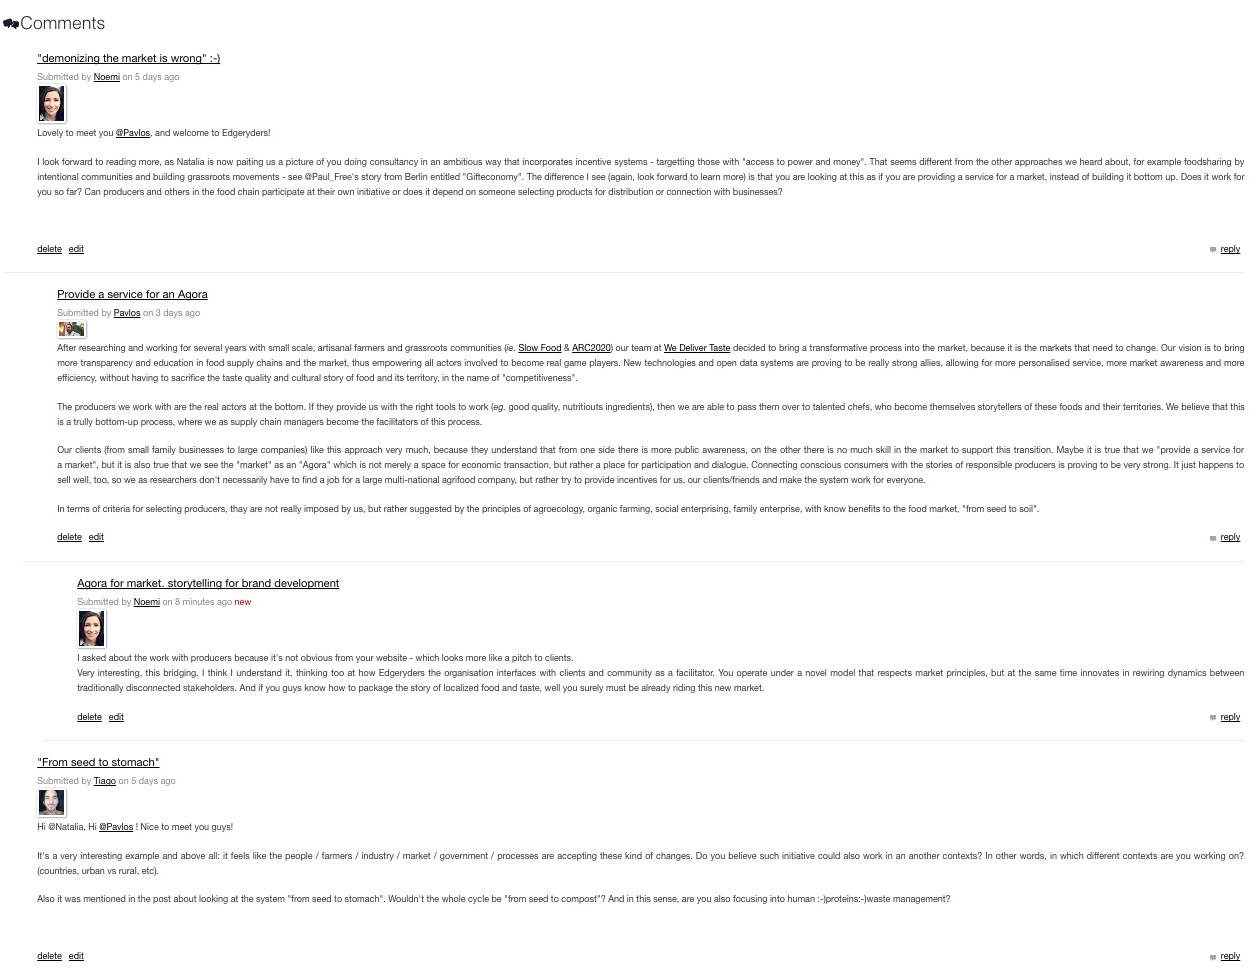
\includegraphics[width= 1 \textwidth]{Threaded_comments_Edgeryders}
	\caption{Threaded comments in the Edgeryders online community. Each comment is in turn commentable. This is represented visually by nested indentation: "sibling" comments (comments to the same post or comment) are visualized in chronological order, with the same level of indent. "Children" comments are visualized directly under their "parent", indented with respect to it.}
	\label{fig:threadedComments}
\end{figure}

We extracted a snapshot of the database on October 7th 2015. At the time, the community had 2,904 registered users, who had authored 4,062 posts and 18,285 comments. 23 of the users had, at some point in time, reported to the Edgeryders company; we cast them as the online community managers for this particular community. 	

All events in our dataset (creating accounts, creating posts, creating comments) are timestamped. This allows for the possibility of modelling interaction in the online community dynamically. 

\subsection{A network model of interaction in online communities}

We need to consider carefully how we incorporate dynamics in our model (\cite{holme2012temporal}). We make the following assumptions:

\begin{enumerate}
	\item The duration of interactions is negligible. This means that events can be represented by a contact sequence, i.e. triples $(i, j, t)$ where $i, j \in V$, the set of interactants (represented as vertices in the network) and $t$ denotes time. This is a standard assumption in studies of person-to-person communication online (\cite{holme2012temporal}). 
	\item First-time interaction produces a permanent change in the social relationship between the source and the target of the interaction (the author and the recipient of the comment). All Edgeryders users can be assumed to share some common interests around social innovation, that motivated them to join Edgeryders. When they interact directly, however, they begin to unpack and specify such common interests, and they (often explicitly) signal interest in each other's activities. This produces a shift in the nature of the relationship between the interacting, which becomes one of actual, as opposed to potential, interaction. Mathematically, this translates into representing interaction by a network whose edges do not decay.
	\item Subsequent interaction also carry social significance. They have the effect of further strengthening the relationship between the two interactants. The strength of the relationship increases monotonically with the number of interactions recorded. The effect of all  interactions after the first one, too, is permanent. Mathematically, this translates into representing interaction by a weighted network.
\end{enumerate}

We then proceeded to build a social network of the interactions within the community as follows:

\begin{enumerate}
	\item Users that have posted at least one post or one comment are included as nodes in the network.
	\item We interpret each comment as one interaction event. Whenever a comment is posted, an edge is induced. The new edge's source node is the node associated to the author of the comment. The new edge's target node is the node associated to the author of the post or comment being commented. 
	\item If an edge with the same source and target already exist, we do not add a new one, but rather increase the edge's weight by one.
	\item If the source and target of the edge are the same, the edge is discarded.  
	\item The sequence of timestamped interaction events allows us to model interaction in Edgeryders as an evolving network. We divide the observation period in one week-long intervals, and consider users to be acting on the basis of the interaction network that they find themselves in at that period. In other words, we do not attempt to model explicitly the entire sequence of interactions; rather, we assume that all agents make simultaneous decisions on who to interact with at the beginning of each time period, and that those decisions are based on the snapshot of the network at the beginning of said period. This means we are following the tradition of literature on evolving networks (\cite{dorogovtsev2002evolution}) rather than that of temporal networks (\cite{holme2012temporal}). This reflects our preoccupation with topological aspects over temporal ones. We claim the choice is justified under the terms suggested by Holme and Saramaki (\cite{holme2012temporal}) \footnote{" [...] a contact sequence that is fairly well modeled by a weighted graph with the assumption that contact times are random, with a frequency proportional to the edge weight"} .

\end{enumerate}

This process results in a sequence of 212 networks, each one a step on the growth path of the interaction network in Edgeryders. At the end of week 1 the network had only 6 nodes and 1 edge; at the end of week 212 it had 789 nodes and 4,861 edges.

\begin{figure}
	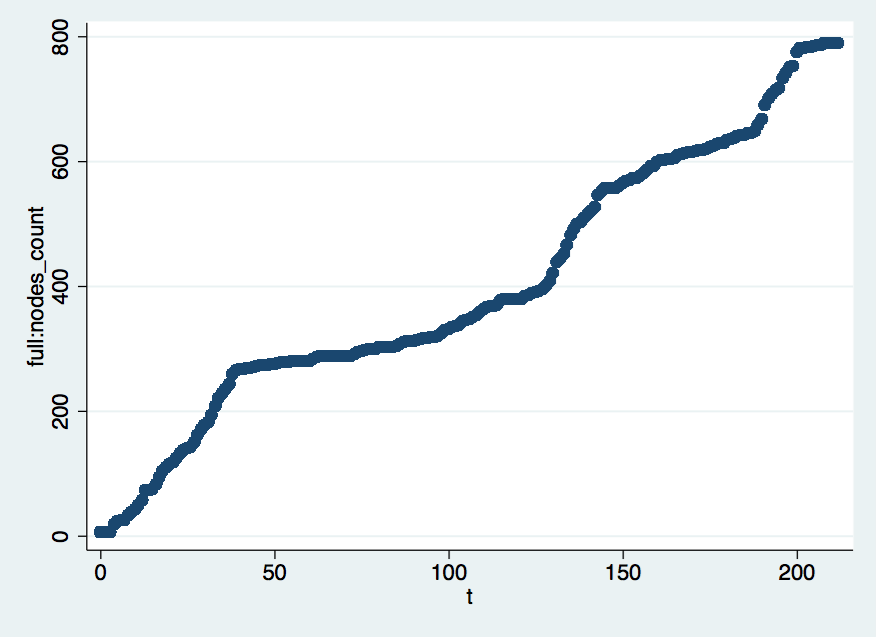
\includegraphics[width=.8 \textwidth]{numnodes}
	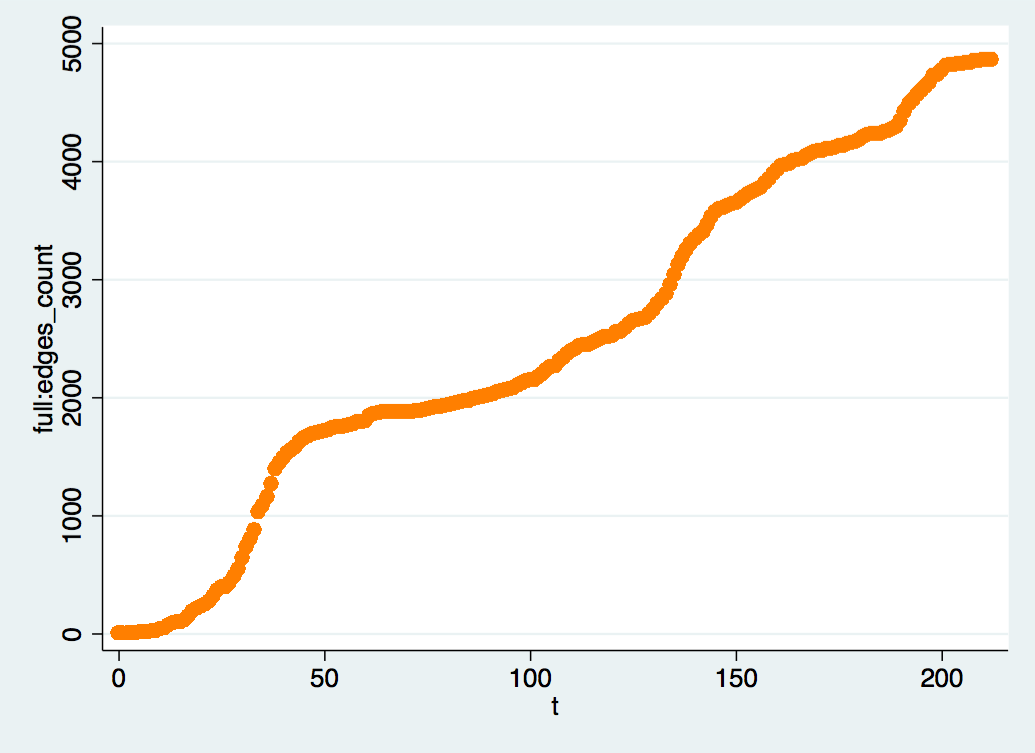
\includegraphics[width=.8 \textwidth]{numedges}
	\caption{Growth of the number of nodes (top) and edges (bottom) in the Edgeryders interaction network.}
\label{fig:growthNodesEdges}
\end{figure}

\subsection{Model}

We model user activity in an online community as a function of three groups of variables:

\begin{equation}
	A_{i,t} = f(NN_{i,t}, EN_{i,t}, GN_t) 
	\label{eq:model}
\end{equation}

Where:
\begin{itemize}
\item $A_{i,t}$ denotes the activity of user $i$ at time $t$, defined as the number of posts plus the number of comments authored by user $i$ during the period.
\item $NN_{i,t}$ denotes a vector of non-network variables associated with user $i$ at time $t$. These include writing a post or a comment; receiving a comment from a community manager; receiving a comment from another user who is not a community manager; the total number of posts and comments written by other users users $A_{j,t}, j \neq i$; and $i$'s experience as a user of Edgeryders, as measured by the number of weeks elapsed since she joined the community. The week of joining can predate the week in which the user writes her first post or comment. 
\item $EN_{i, t}$ denotes a vector of variables pertaining to the user's ego network at time $t$. These include her own in-degree (the number of users linking to her); her out-degree (the number of users she links to); her betweenness centrality (the fraction of shortest paths across any two users $j,k \neq i$ that $i$ finds herself on); her PageRank (the probability that a random walker across the network would end up at this particular node\footnote{PageRank was originally developed as a measure of network centrality for the World Wide Web (\cite{brin2012reprint}).}; and her clustering coefficient (the fraction of $i$'s neighbours that are also neighbours to each other).
\item $GN_{i,t}$ denotes a vector of variables pertaining to the global network at time $t$. These include the total number of nodes; the total number of edges; the average degree; and the network's Louvain modularity\footnote{The modularity of a network is a measure of how much it differs from an Erdos-Renyi random network with the same degree distribution. Values close to 0 indicate it is indistinguishable from a random network; values close to -1 or 1 indicate structure (\cite{clauset2004finding}). Measuring modularity is computationally hard; it is customary to use algorithms to compute an approximate value. Of these, the Louvain algorithm is the most widely used in the literature for its attractive computational efficiency \cite{blondel2008fast}.  }.
\end{itemize}

\subsection{Estimation}

We estimate the behaviour of a binary variable $A_{i,t}$ that takes value $1$ if user $i$ engages actively in interaction (i.e. writes a post or a comment at time $t$), and $0$ otherwise. We make use of a logit model:

\begin{equation}
	PR(A_{i,t}= 1|X_{i,t}) = \frac{e^{X_{i,t}\beta}}{1 + e^{X_{i,t}\beta}}
	\label{eq:estimation}
\end{equation}

Where $X_{i,t}$ is a vector of observed explanatory variables; $\beta$ is a vector of parameters.

An advantage of the logit model is that its coefficient lend themselves to being interpreted in terms of marginal effects on the log-odds ratio (\cite{cameron2005microeconometrics}). We rewrite equation \ref{eq:estimation} as

\begin{equation}
	ln \frac{Pr(A_{i,t} = 1)}{1 - Pr(A_{i,t}=1)} = X_{i,t} \beta 
	\label{eq:logOdds}
\end{equation}

Next, we proceed to estimating equation \ref{eq:logOdds} with fixed effects on the 766 Edgeryders users who have no moderator or site administrator role. To do this, we drop the 23 users that have such roles. We add to the right hand-side
$c_i$, an unobserved time-invariant effect specific to user $i$; this is intended to get rid of the bias introduced by different individuals having a different propensity to participate in the online conversation, as this is likely to be correlated with some of the regressors\footnote{For example, it is possible that "chattier" individuals might end up with higher in- and -out degrees, higher network centrality, and so on. }. We also add $u_{i,t}$, a residual error term, with mean zero and uncorrelated with right-hand side variables. We take care to employ lagged variables when failure to do so might cause endogeneity issues. 

\begin{equation}
	ln \frac{Pr(A_{i,t} = 1)}{1 - Pr(A_{i,t}=1)} = X_{i,t} \beta + c_i + u_{i,t}
	\label{eq:logOddsErrors}
\end{equation}

\subsection{Software stack}
Primary data from the Edgeryders database were obtained using a Drupal plugin called Views JSON. We used a modified version of an application software called Edgesense\footnote{\url{https://github.com/Wikitalia/edgesense}. Modifications added support for computing some extra network metrics, like the clustering coefficient.} to build a network representation of the interaction in Edgeryders. We then enriched the data so obtained with non-network metrics computed directly from the primary data, and exported the results in tabular form. Such results were then imported into Stata for estimation. 

Code and data are available at the following address: (redacted to guarantee author's anonymity).
